\subsubsection{Q10.20 data 10312021 11092021 grouped by scenario \& PGM}

\begin{comment}
                             EFPR        EO      EFNR     n    pvalue
(frauth, Advantaged)     0.515152  0.484848  0.439394  33.0  0.868044
(frauth, Disadvantaged)  0.400000  0.600000  0.500000  10.0  0.556267
(icu, Advantaged)        0.710526  0.289474  0.578947  19.0  0.016855
(icu, Disadvantaged)     0.500000  0.500000  0.676471  17.0  1.000000
(rent, Advantaged)       0.218750  0.781250  0.437500  16.0  0.006561
(rent, Disadvantaged)    0.521739  0.478261  0.521739  23.0  0.646777
\end{comment}

\begin{table}[h]
    \centering
    \begin{tabular}{|c|c|c|c|c|c|c|}
        \hline
        scenario & PGM & EFPR & EO & EFNR & n & p-value\\
        \hline
        frauth & Advantaged & \textbf{0.515} & 0.485 & 0.439 & 33.0 & 0.868\\
		frauth & Disadvantaged & 0.400 & \textbf{0.600} & 0.500 & 10.0 & 0.556\\
		icu & Advantaged & \textbf{0.711} & 0.289 & \textbf{0.579} & 19.0 & \textbf{0.017}\\
		icu & Disadvantaged & 0.500 & 0.500 & \textbf{0.676} & 17.0 & 1.000\\
		rent & Advantaged & 0.219 & \textbf{0.781} & 0.438 & 16.0 & \textbf{0.007}\\
		rent & Disadvantaged & \textbf{0.522} & 0.478 & \textbf{0.522} & 23.0 & 0.647\\
		
        \hline
    \end{tabular}
    \caption{Grouped by scenario PGM}
    \label{tab:my_label}
\end{table}
\begin{figure}[h]
    \centering
    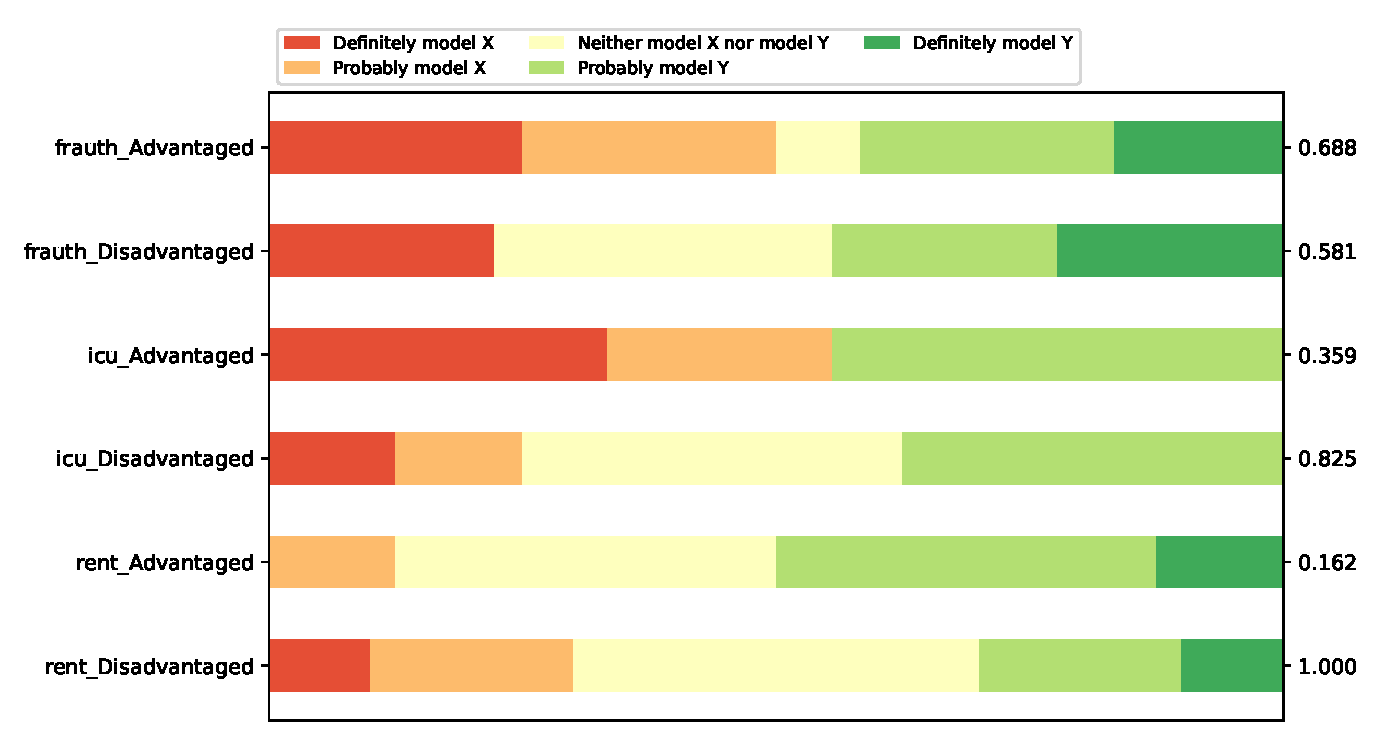
\includegraphics[width=0.8\textwidth]{figures/Q10.20/10312021_11092021/Q10.20_scenario_PGM.pdf}
    \caption{Grouped by scenario \& PGM}
    \label{fig:my_label}
\end{figure}
